\documentclass[12pt,a4paper,openright,twoside]{book}
\usepackage[utf8]{inputenc}
\usepackage{disi-thesis}
\usepackage{code-lstlistings}
\usepackage{notes}
\usepackage{shortcuts}
\usepackage{acronym}

\school{\unibo}
\programme{Corso di Laurea Magistrale in Ingegneria e Scienze Informatiche}
\title{MYOP - Make your own poll \\
Libreria multipiattaforma \\
a supporto della \\
democrazia digitale
}
\author{Jacopo Corina}
\date{\today}
\subject{Laboratorio di sistemi software}
\supervisor{Prof. Danilo Pianini}
\session{III}
\academicyear{2022-2023}

% Definition of acronyms
\acrodef{IoT}{Internet of Thing}
\acrodef{vm}[VM]{Virtual Machine}


\mainlinespacing{1.241} % line spacing in mainmatter, comment to default (1)

\begin{document}

\frontmatter 
\frontispiece

\begin{abstract}	
Max 2000 characters, strict.
\end{abstract}

\begin{dedication} % this is optional
Ai miei genitori
\end{dedication}

\begin{acknowledgements} % this is optional
Optional. Max 1 page.
\end{acknowledgements}

%----------------------------------------------------------------------------------------
\tableofcontents   
\listoffigures     % (optional) comment if empty
\lstlistoflistings % (optional) comment if empty
%----------------------------------------------------------------------------------------

\mainmatter

%----------------------------------------------------------------------------------------
\chapter{Introduzione}
\label{chap:introduction}
%----------------------------------------------------------------------------------------
\chapter{Democrazia digitale}
Qua farei un recap delle piattaforme esistenti, ponendo l'accento sul fatto
che sono poco specifiche ed adattabili. Inoltre non sono librerie e il
funzionamento è abbastanza nascosto ai non addetti ai lavori
\section{Stato dell' arte}
%----------------------------------------------------------------------------------------
\chapter{Automazione e versionamento artefatti}

\section{Kotlin Multiplatform}
Spiegare brevemente in cosa consiste, con immagini a supporto

\section{Github}

    \subsection{Github Actions}
    Spiegazione funzionamento pipelines

    \subsection{Github Pages}
    Hosting di documentazione

    \subsection{Artefatti}
    Nota per il Prof.
    Non so se va spiegata qui la pubblicazione su Maven central/ github packages / npm
    oppure se parlarne direttamente nell' implementazione
%----------------------------------------------------------------------------------------
\chapter{Analisi}
In questa parte metterei dettagli su votazioni a singola preferenza 
e votazioni a lista di preferenze (es.Condorcet)
\section{Requisiti}

    \subsection{Requisiti funzionali}

    \subsection{Requisiti non funzionali}

\section{Modello del dominio}
%----------------------------------------------------------------------------------------
\chapter{Design}
%----------------------------------------------------------------------------------------
\chapter{Implementazione}

\section{Librerie multiplatform utilizzate}

\section{Pubblicazione di artefatti}
Spiegare brevemente i passaggi necessari che sono stati fatti per arrivare
alle pubblicazioni

\section{Pubblicazione della documentazione}
spiegare la creazione di un nuovo workflow, e collegato a quelli esistenti
%----------------------------------------------------------------------------------------
\chapter{Valutazione}

\section{Test realizzati}
Descrivere le varie situazioni che sono andato a controllare,
mettendo dettagli solo per i casi più complicati

\section{Sperimentazione con Ergast API}
Estratti di demo che ho realizzato usando i dati della Formula 1
%----------------------------------------------------------------------------------------
\chapter{Conclusioni}




%Write your intro here.
%\sidenote{Add sidenotes in this way. They are named after the author of the thesis}

%You can use acronyms that your defined previously,
%You can use acronyms that your defined previously,
%such as \ac{IoT}.
%
%If you use acronyms twice,
%they will be written in full only once
%(indeed, you can mention the \ac{IoT} now without it being fully explained).
%
%In some cases, you may need a plural form of the acronym.
%
%For instance,
%that you are discussing \acp{vm},
%you may need both \ac{vm} and \acp{vm}.

%\paragraph{Structure of the Thesis}

%\note{At the end, describe the structure of the paper}

%\chapter{State of the art}

%I suggest referencing stuff as follows: \cref{fig:random-image} or \Cref{fig:random-image}

%\begin{figure}
%    \centering
%    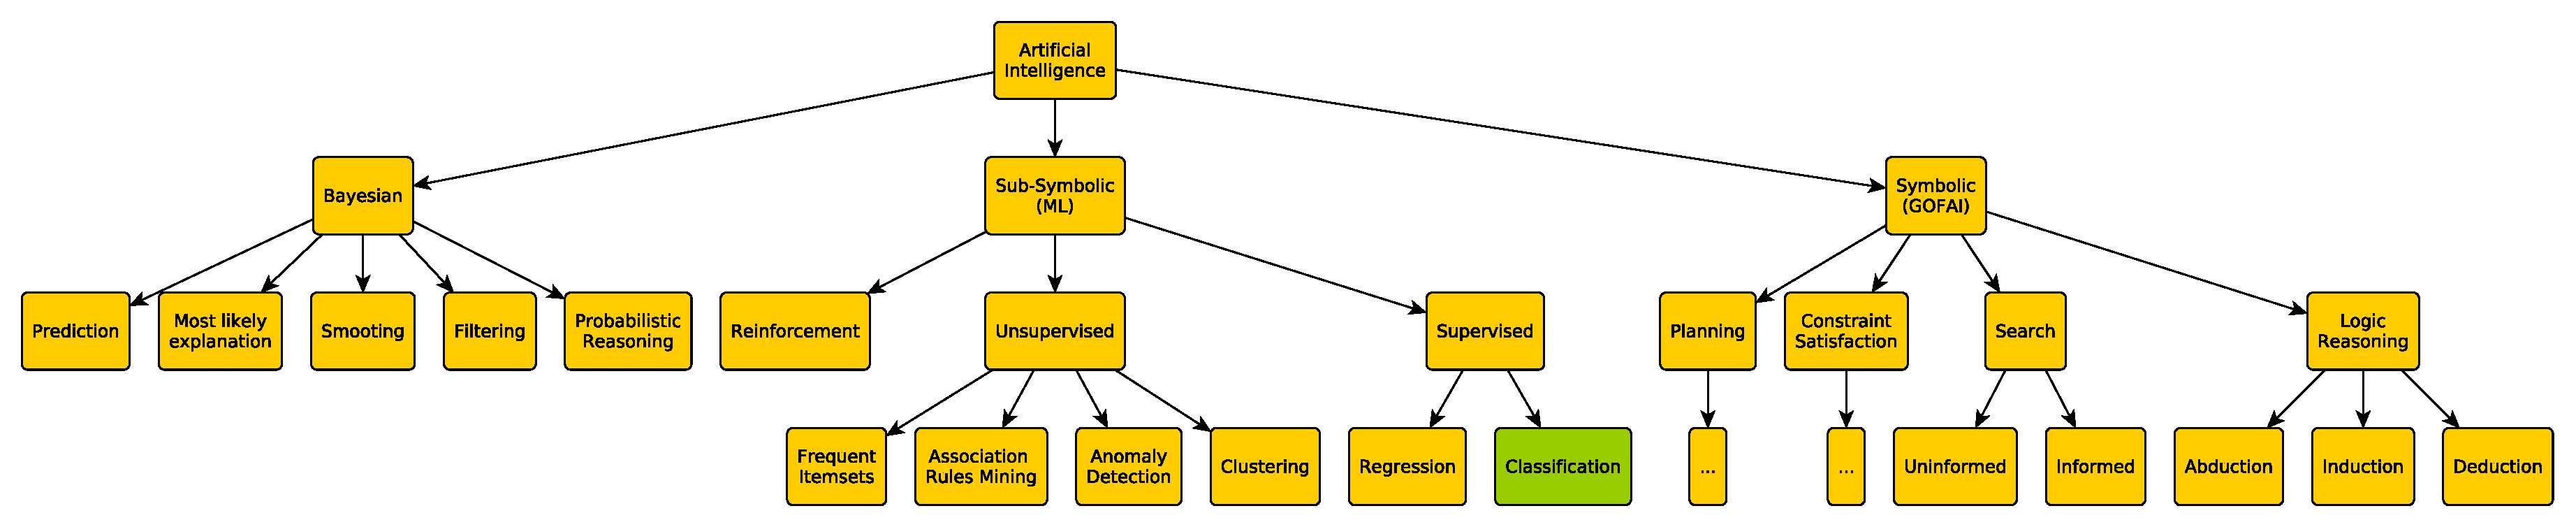
\includegraphics[width=.8\linewidth]{figures/random-image.pdf}
%    \caption{Some random image}
%    \label{fig:random-image}
%\end{figure}

%\section{Some cool topic}

%\chapter{Contribution}

%You may also put some code snippet (which is NOT float by default), eg: \cref{lst:random-code}.

%\lstinputlisting[float,language=Java,label={lst:random-code}]{listings/HelloWorld.java}

%\section{Fancy formulas here}

%----------------------------------------------------------------------------------------
% BIBLIOGRAPHY
%----------------------------------------------------------------------------------------

\backmatter

\nocite{*} % comment this to only show the referenced entries from the .bib file


\bibliographystyle{alpha}
\bibliography{bibliography}

\end{document}